%%%%%%%%%%%%%%%%%%%%%%%%%%%%%%%%%%%%%%%%%
% Short Sectioned Assignment LaTeX Template Version 1.0 (5/5/12)
% This template has been downloaded from: http://www.LaTeXTemplates.com
% Original author:  Frits Wenneker (http://www.howtotex.com)
% License: CC BY-NC-SA 3.0 (http://creativecommons.org/licenses/by-nc-sa/3.0/)
%%%%%%%%%%%%%%%%%%%%%%%%%%%%%%%%%%%%%%%%%

%----------------------------------------------------------------------------------------
%	PACKAGES AND OTHER DOCUMENT CONFIGURATIONS
%----------------------------------------------------------------------------------------

\documentclass[paper=a4, fontsize=11pt]{scrartcl} % A4 paper and 11pt font size

% ---- Entrada y salida de texto -----

\usepackage[T1]{fontenc} % Use 8-bit encoding that has 256 glyphs
\usepackage[utf8]{inputenc}
%\usepackage{fourier} % Use the Adobe Utopia font for the document - comment this line to return to the LaTeX default

% ---- Idioma --------

\usepackage[spanish, es-tabla]{babel} % Selecciona el español para palabras introducidas automáticamente, p.ej. "septiembre" en la fecha y especifica que se use la palabra Tabla en vez de Cuadro

% ---- Otros paquetes ----

\usepackage{url} % ,href} %para incluir URLs e hipervínculos dentro del texto (aunque hay que instalar href)
\usepackage{amsmath,amsfonts,amsthm} % Math packages
%\usepackage{graphics,graphicx, floatrow} %para incluir imágenes y notas en las imágenes
\usepackage{graphics,graphicx, float} %para incluir imágenes y colocarlas

% Para hacer tablas comlejas
%\usepackage{multirow}
%\usepackage{threeparttable}

%\usepackage{sectsty} % Allows customizing section commands
%\allsectionsfont{\centering \normalfont\scshape} % Make all sections centered, the default font and small caps

\usepackage{fancyhdr} % Custom headers and footers
\pagestyle{fancyplain} % Makes all pages in the document conform to the custom headers and footers
\usepackage{eurosym} % Para poder añadir el símbolo del euro
\fancyhead{} % No page header - if you want one, create it in the same way as the footers below
\fancyfoot[L]{} % Empty left footer
\fancyfoot[C]{} % Empty center footer
\fancyfoot[R]{\thepage} % Page numbering for right footer
\renewcommand{\headrulewidth}{0pt} % Remove header underlines
\renewcommand{\footrulewidth}{0pt} % Remove footer underlines
\setlength{\headheight}{13.6pt} % Customize the height of the header

\numberwithin{equation}{section} % Number equations within sections (i.e. 1.1, 1.2, 2.1, 2.2 instead of 1, 2, 3, 4)
\numberwithin{figure}{section} % Number figures within sections (i.e. 1.1, 1.2, 2.1, 2.2 instead of 1, 2, 3, 4)
\numberwithin{table}{section} % Number tables within sections (i.e. 1.1, 1.2, 2.1, 2.2 instead of 1, 2, 3, 4)

\setlength\parindent{0pt} % Removes all indentation from paragraphs - comment this line for an assignment with lots of text

\newcommand{\horrule}[1]{\rule{\linewidth}{#1}} % Create horizontal rule command with 1 argument of height


%----------------------------------------------------------------------------------------
%	TÍTULO Y DATOS DEL ALUMNO
%----------------------------------------------------------------------------------------

\title{	
\normalfont \normalsize 
\textsc{\textbf{Modelos de computación (2017-2018)} \\ Doble Grado en Ingeniería Informática y Matemáticas \\ Universidad de Granada} \\ [25pt] % Your university, school and/or department name(s)
\horrule{0.5pt} \\[0.4cm] % Thin top horizontal rule
\huge Relación de problemas II \\ % The assignment title
\horrule{2pt} \\[0.5cm] % Thick bottom horizontal rule
}

\author{Alberto Jesús Durán López} % Nombre y apellidos

\date{\normalsize\today} % Incluye la fecha actual

%----------------------------------------------------------------------------------------
% DOCUMENTO
%----------------------------------------------------------------------------------------

\begin{document}

\maketitle % Muestra el Título

\newpage %inserta un salto de página

\tableofcontents % para generar el índice de contenidos

%\listoffigures

% \listoftables

\newpage













\section{Ejercicio 17}
\begin{itemize}
	\item \textbf{Diseña un autómata finito determinista que reconozca el siguiente \\ lenguaje:} \\
	$L_{3}$ = \{u $\in$ $\{0,1\}^{*}$ | el número de 1's no es múltiplo de 3 y el número de 0's es par \} \\	
	
	\begin{figure}[h]
		\centering
		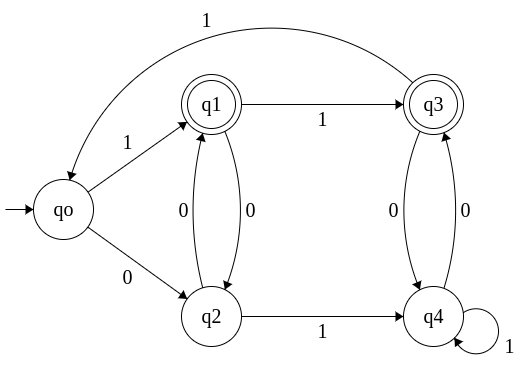
\includegraphics[scale=0.5]{AF.png}
	\end{figure}

\end{itemize} 





\section{Ejercicio 22}

\begin{itemize}
	\item \textbf{Dar una expresión regular para el lenguaje aceptado por el siguiente autómata:}
	
	\begin{figure}[h]
		\centering
		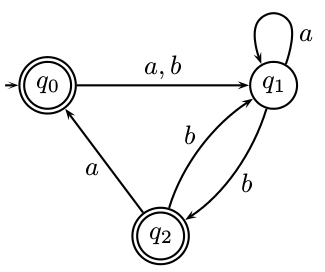
\includegraphics[scale=0.5]{22.png}
	\end{figure}
	
	Dicho autómata posee una expresión regular dada por:
	
	( (a+b)a*b (ba*b)* (a+$\epsilon$) )*
	
\end{itemize}







\newpage
\section{Ejercicio 23}
\begin{itemize}
	\item \text{Sea $B_n = \{a^{k} $| k múltiplo de n\}. Demostrar que $B_n$ es regular para todo n}.
	\begin{center}
		Sea k=nm, entonces: \\
		$a^{k} = a^{nm} = (a^{n})^{m} = (a^{n})^{*} $, por tanto es regular
	\end{center}
\end{itemize}



\section{Ejercicio 24}
\begin{itemize}
	\item \textbf{Decimos que u es un prefijo de v si existe un w tal que uw=v. Decimos que u es un prefijo propio de v si además u $\not=$ v y u $\not =$ $\epsilon$. Demostrar que si L es regular, también lo son los lenguajes: \\ \\
	a)NOPREFIJO(L) =\{u$\in$L | ningún prefijo propio de u pertenece a L\} \\ \\
	b) NOEXTENSION(L) = \{u$\in$L | u no es prefijo propio de ninguna \\ palabra de L\}
	}
	
	a)Si u$\in$L, entonces u=vw donde v no es prefijo propio. Es decir, v $\not=$ u y v$\not=$$\epsilon$ por lo que es la concatenación de dos palabras, para todo u $\in$L, por tanto es regular.
	
	b) Como u no es prefijo propio de ninguna palabra de L, sea una palabra v $\in$ L, u=v por lo que u$\in$ L y como L era regular, NOEXTENSION(L) también es regular.
	
\end{itemize}

\newpage
\section{Ejercicio 25}
\begin{itemize}
	\item \textbf{Si L $\subseteq$ $A^{*}$, define la relación $\equiv$ en $A^{*}$ como sigue: si u,v $\in$ $A^{*}$, entonces \\u $\equiv$ v si y solo si para toda z $\in$ $A^{*}$, tenemos que (xz $\in$ L $\Longleftrightarrow$ yz $\in$ L)}\\
	\\a) Demostrar que $\equiv$ es una relación de equivalencia
	\\b) Calcular las clases de equivalencia de L=\{ $a^{i}b^{i}$ | i $\geq$ 0\}
	\\c)Calcular las clase de equivalencia de L=\{ $a^{i}b^{j}$ | i,j $\geq$ 0\}
	\\d) Demostrar que L es aceptado por un autómata finito determinista si y solo si el número de clases de equivalencia es finito.
	\\e) ¿Qué relación existe entre el número de clases de equivalencia y el autómata finito minimal que acepta L?
	
	
\end{itemize}

a) Para comprobar que es una relación de equivalencia comprobamos las siguientes \\propiedades:
\begin{itemize}
\item \textbf{Reflexiva:   x $\sim$ x \\ }
xz  $\in$ L $\Longleftrightarrow$ xz $\in$ L

\end{itemize}

\begin{itemize}
\item \textbf{Simétrica:\\}
x $\sim$ y:  xz $\in$ L $\Longleftrightarrow$ yz $\in$ L
\\y $\sim$ x: y'z $\in$ L $\Longleftrightarrow$ x'z $\in$ L  ,  $\hspace{1cm}$ Restamos:
\\ xz -y'z = yz-x'z
\\(x-y')z=(y-x)z
\\x-y'=y-x' $\Longleftrightarrow$ x=y' $\hspace{0.5cm}$ y $\hspace{0.5cm}$ y=x' $\hspace{1cm}$ Por tanto:
\\ x $\sim$y =y$\sim$x

\end{itemize}

\begin{itemize}
\item \textbf{Transitiva: \\}
x $\sim$ y: xz $\in$ L $\Longleftrightarrow$ yz $\in$ L
\\y $\sim$ z': yz $\in$ L $\Longleftrightarrow$ z'z $\in$L
\\x $\sim$ z': xz $\in$ L $\Longleftrightarrow$ z'z $\in$ L $\hspace{1cm}$ Por tanto:

x $\sim$ y + y $\sim$z'
\\xz + yz = yz+z'z
\\(x+y)z=(y+z')z
\\x+y=y+z'
\\x=z' $\Longleftrightarrow$ x$\sim$z'

\end{itemize}

\newpage
b) \\
\scalebox{1}[1]{
	\begin{tabular}{|r|l|l|}
		\hline
		i=1&ab \\
		\hline
		i=2& aabb \\
		\hline
		i=3& aaabbb  \\
		\hline
		i=4& aaaabbbb \\
		\hline
		i=n& a...$a_n$b...$b_n$ \\
		\hline
	\end{tabular}} \\
	
Según la relación de equivalencia, dos palabras están relacionadas si tienen el mismo sufijo z $\in$ $A^{*}$, por lo que para este lenguaje, cada palabra generada para cada i $\in$ N, sólo está relacionada consigo misma por lo que en total habrá n clases de equivalencia. \\




c) \\
\scalebox{1}[1]{
	\begin{tabular}{|r|l|l|l|l|l|}
		\hline
		&j=0 &j=1 &j=2 &j=3 &j=4\\
		\hline
		i=1& a &ab &abb &abbb &abbbb\\
		\hline
		i=2& aa &aab &aabb &aabbb &aabbbb\\
		\hline
		i=3& aaa& aaab &aaabb &aaabbb &aaabbbb\\
		\hline
	\end{tabular}}\\

-Si i>0, j > 0: \\
Para este otro lenguaje, todas las palabras con el mismo valor de j están relacionadas ya que comparten el mismo sufijo por lo que habrán un total de j clases de equivalencia.
\\ -Si i=0 ó j=0, hay únicamente 1 clase de equivalencia.
\\-Si i=0 y j=0, no hay clases de equivalencia. \\

d)L es aceptado por un automata finito determinista si es regular. Si L es regular el numero de clases de equivalencia es finito por lo que queda demostrado que si L es \\aceptado por un automata finito determinista entonces el numero de clases de \\equivalencia es finito.\\



e) Cada clase de equivalencia corresponde a un estado en el AFD minimal





\end{document}